\documentclass{article}

\usepackage{amsfonts}
\usepackage{amsmath}
\usepackage{amssymb}
\usepackage{amsthm}
\usepackage{bookmark}
\usepackage{cancel}
\usepackage{extramarks}
\usepackage{fancyhdr}
\usepackage{floatrow}
\usepackage{forest}
\usepackage{graphicx}
\usepackage{hyperref}
\usepackage{listings}
\usepackage{mathrsfs}
\usepackage{proof}
\usepackage{pythonhighlight}
\usepackage[doublespacing]{setspace}
\usepackage{textcomp}
\usepackage{tikz}
\usepackage{wrapfig}
\usepackage{xparse}
\usepackage{xstring}
\usepackage{mathtools}
\usepackage{indentfirst}
\usepackage{hanging}

\usepackage[backend=biber]{biblatex}
\addbibresource{APPMProject.bib}

\usetikzlibrary{automata,positioning}

%
% Basic Document Settings
%

\topmargin=-0.45in
\evensidemargin=0in
\oddsidemargin=0in
\textwidth=6.5in
\textheight=9.0in
\headsep=0.25in

\linespread{1.1}

\pagestyle{fancy}



\lhead{\textit{APPM 4360}}
\rhead{Final Project}
\lfoot{\lastxmark}
\cfoot{\thepage}

\renewcommand\headrulewidth{0.4pt}
\renewcommand\footrulewidth{0.4pt}

% \setlength\parindent{0pt}



 

%
% Title Page
%

\title{
	
}

\author{\hmwkAuthorName}
\date{}

%
% Various Helper Commands and Formatting Directives
%

\doublespacing

\allowdisplaybreaks

\title{Propagation of Voltage in a Neuron}
\author{Jamie George, Francesca Sica, Eric Wilkinson}
\date{December 7, 2020}

\begin{document}

\begin{titlepage}
    
    \begin{center}
        \vspace*{2cm}
        
        \Huge
        \textbf{Applications of Schwarz-Christoffel Transformations}
        
        \vspace*{1cm}
        
        \large
        \textbf{Jamie George}
        
        \vspace{1cm}
        
        \Large
        \textbf{University of Colorado Boulder}
        
        \vspace{1cm}
        
        \Large
        \textbf{Department of Applied Mathematics}
        
        \vspace{1cm}
        
        \Large
        \textbf{26 April 2021}
        
    \end{center}
    
\end{titlepage}


\pagebreak

\section{Abstract}
Schwarz-Christoffel transformations are a useful conformal mapping technique that allows one to map regions interior or exterior to a polygon to the upper half of another plane. This type of transformation is particularly useful as it allows an object with inconvenient geometry in one domain to be conformally mapped to a more convenient domain. This paper will examine how Schwarz-Christoffel transformations can be used to conformally map semi-infinite polygonal regions.

\section{Introduction}
The Schwarz-Christoffel mapping is a specific type of conformal mapping. In general, a conformal mapping is a transformation \(w = f(z)\) that preserves the angle between differentiable arcs (Ablowitz \& Fokas, 2003). The transformation \(w = f(z)\) may be understood as the mapping of the domain $D$ onto the domain \(D^{*}=f(D)\). An important concept concerning conformal mappings is Riemann’s Mapping Theorem. Riemann’s Mapping Theorem declares that any simply connected domain of the $z$ plane, except the entire z plane or extended z plane, can be mapped with a transformation \(w = f(z)\) onto a disk \(|w| < 1\). While this statement is useful, it does not explicitly give us a way to find \(f(z)\). Finding \(f(z)\) is where the Schwarz-Christoffel transformation comes in. 

The Schwarz-Christoffel transformation allows one to map the upper half of the $z$ plane and the interior (or exterior) of a polygon in the $w$ plane. This transformation makes use of the Schwarz reflection principle. This principle allows us to take an analytic function \(f(z)\) defined in the upper half-plane and extend it to the lower half-plane (Ablowitz \& Fokas, 2003). The function \(f(z)\), analytic in a domain D, can be extended to the lower half-plane, domain \(\tilde{D}\), by the formula \(f(\tilde{z}) = \overline{f(\bar{z})}\). 

In this project, the Schwarz-Christoffle transformation will be used to conformally map semi-infinite polygonal regions. We will first consider a semi-infinite strip. In general, semi-infinite strips may be treated as triangles with one infinite vertex (Driscoll \& Trefethen, 2002). Following this an infinite strips will be considered. Infinite strips are treated as a rhombus with two infinite vertices. 

\section{Description}
\subsection{Schwarz-Christoffel Theorem}
        In this project, the Schwarz-Christoffel transformation will be used to map a polygonal boundary in the $w$ plane into the real-axis of the $z$ plane. 
        Let \(\Gamma\)  define the piecewise linear boundary of a polygon in the $w$ plane with interior angles \(\alpha_{1}\pi,\alpha_{2}\pi,...,\alpha_{n}\pi\) (Ablowitz \& Fokas, 2003). The transformation is defined by the equation 
        
        \begin{equation}
            \frac{dw}{dz} = \gamma(z-a_{1})^{\alpha_{1} - 1}(z-a_{2})^{\alpha_{2} - 1}\cdots (z-a_{n})^{\alpha_{n}-1}
        \end{equation}
        
        where \(\gamma\) is a complex number and \(a_{1}, a_{2}, \ldots, a_{n}\) are real values. The vertices of the polygon in the $w$ plane, $A_{1}, A_{2}, ..., A_{n}$, are mapped to the points $a_{1}, a_{2}, ..., a_{n}$ on the real axis of the $z$ plane. Figure 1 demonstrates this relationship. 
        
        \begin{figure}
            \centering            
            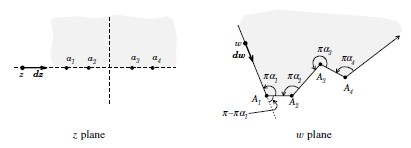
\includegraphics[scale = 1.5 ]{Schwarz christoffle mapping.jpg}
            \caption{Schwarz-Christoffle Transformation}
            \label{fig:my_label}
        \end{figure}
        
        The interior angle at a vertex $j$ is defined as the change of angle from the outgoing side at \(A_{j}\) to the incoming side (Driscoll \& Trefethen, 2002). For a finite vertex \(A_{j}\) we have \( \alpha_{j} \in (0, 2]\). If the vertex \(A_{j}\) is the tip of a slit, then \(\alpha_{j} = 2\). Furthermore recall that the turns around any closed polygon must sum to \(2\pi\), thus, for a polygon with $n$ sides, we have
        
        \begin{equation}
            \sum_{l = 1}^{n} \alpha_{l} = n - 2
        \end{equation}
        
        In the following applications, one or more of the vertices of the polygon will correspond to infinity. Suppose the point \(w = A_{1}\) is an infinite vertex. In this case, \((z-a_{1})\) becomes effectively a constant and can be absorbed into a new constant \(\hat{\gamma}\) (Fitzpatrick, 2016). This simplification produces the new transformation
        
        \begin{equation}
            \frac{dw}{dz} = \hat{\gamma}(z-a_{2})^{\alpha_{2} - 1}(z-a_{3})^{\alpha_{3} - 1}\cdots (z-a_{n})^{\alpha_{n}-1}
        \end{equation}
    

\subsection{Semi-Infinite Strip}
  For the first application, we will examine semi-infinite strips. Semi-infinite strips are treated as triangles with one infinite vertex (Driscoll \& Trefethen, 2002). From equation 2 we have \(\alpha_{1} + \alpha_{2} + \alpha_{3} = 1\). If we take the infinite vertex to be $A_{1}$, then we have \(\alpha_{1} = 0\) and \(\alpha_{2} = \alpha_{3} = \frac{1}{2}\). Now, we may consider a vertically oriented semi-infinite strip of width \(2d\) located in the $w$ plane, as seen in figure 2.
    
    \begin{figure}
        \centering            
        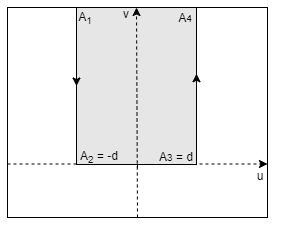
\includegraphics[scale = .75 ]{Verticle strip.png}
        \caption{Vertical Semi-Infinite Strip in the $w$ plane}
        \label{fig:my_label}
    \end{figure}
    
    In this example, the semi-infinite strip will be conformally mapped to the upper half of the $z$ plane. The infinite vertex \(A_{1}\) in the $w$ plane corresponds to the infinite point \(a_{1}\) in the $z$ plane (Ablowitz \& Fokas, 2003). The vertex \(A_{2} = -d\) in the $w$ plane corresponds to the point \(a_{2} = -1\) in the $z$ plane. Likewise, the vertex \(A_{3} = d\) corresponds to \(a_{3} = 1\). Furthermore, using the Schwarz reflection principle, we may also conclude that the infinite vertex \(A_{4}\) corresponds to the infinite point \(a_{4}\). Using equation (3) we obtain the relation
    
    \begin{equation}
        \frac{dw}{dz} = \frac{\hat{\gamma}}{\sqrt{(z-1)(z+1)}} = \frac{\tilde{\gamma}}{\sqrt{1-z^{2}}}
    \end{equation}
    
    Integration yields the result
    
    \begin{equation}
        w = \tilde{\gamma} \ sin^{-1}(z) + c
    \end{equation}
    
    Note that \(sin(-1) = -\frac{\pi}{2}\) and \(sin(1) = \frac{\pi}{2}\) thus \(c = 0\) and \(\tilde{\gamma} = \frac{2d}{\pi}\). Substituting the constants into equation (5) gives us the relation \(w = \frac{2d}{\pi}sin^{-1}(z)\). This transformation maps a vertically oriented semi-infinite strip in the $w$ plane onto the upper half of the $z$ plane, as displayed in figure 3. 
    
    In the case of a horizontally oriented strip, as seen in figure 4, the derivation of the transformation is very similar. The infinite vertex \(A_{1}\) in the $w$ plane corresponds to the infinite point \(a_{1}\) in the $z$ plane, \(A_{2} = di\) corresponds to \(a_{2} = - 1\), \(A_{3} = -di\) corresponds to \(a_{3} = 1\), and the infinite vertex \(A_{4}\) corresponds to the infinite point \(a_{4}\). From equation (3) we obtain 
    
    \begin{figure}
        \centering            
        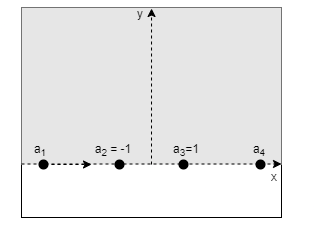
\includegraphics[scale = .75 ]{Vertivle strip z-plane.png}
        \caption{Vertical Semi-Infinite Strip mapped to $z$ plane}
        \label{fig:my_label}
    \end{figure}
    

    
    \begin{equation}
        \frac{dw}{dz} = \frac{\bar{\gamma}}{\sqrt{z^{2} - 1}}
    \end{equation}
    \\
    \\
    
    After integrating and solving for the constants we get the result
    
    \begin{equation}
        w = \frac{2d}{\pi} \ cosh^{-1}(z) - di
    \end{equation}
    Note that this horizontally oriented semi-infinite strip maps onto the upper half of the $z$ plane (see figure 3). This mirrors what happened with a vertically oriented semi-infinite strip.  

\subsection{Infinite Strip} 
    Now we will consider the Schwarz-Christoffel mapping for an infinite strip located in the $w$ plane. Note that an infinite strip can be treated as a polygon with two infinite vertices. Using equation (2) we have that \(\alpha_{1} + \alpha_{2} = 0\). Since both vertices are at infinity, we have \(\alpha_{1} = \alpha_{2} = 0\) (Driscoll \& Trefethen, 2002). The Schwarz-Christoffel transformation then takes the form 
    \begin{equation}
        w = \hat{\gamma} \ ln(z-a_{1}) + c
    \end{equation}
    In this example, suppose the strip has a width of d. When determining this transformation, it is convenient to consider the strip as a limiting form of a rhombus (Bergonio, 2007), as seen in figure 4. 
    \begin{figure}
        \centering            
        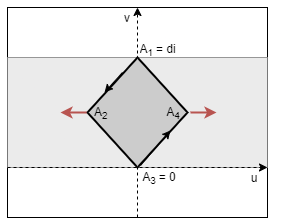
\includegraphics[scale = 0.75]{Infinite channel- rhombus (2).png}
        \caption{Rhombus in $w$ plane}
        \label{fig:my_label}
    \end{figure}
    In this case, \(\alpha_{1} = \alpha_{3} = 1\) and \(\alpha_{2} = \alpha_{4} = 0\). Now, note that only three of the prevertices can be arbitrarily prescribed (Ablowitz\& Fokas, 2003). Let \(a_{2} = 0\), \(a_{3} = 1\), and \(a_{4} = \infty\).  
    From equation (3) we obtain the relation
    \begin{equation}
        \frac{dw}{dz} = \frac{\hat{\gamma}}{z}
    \end{equation}
    Integration yields
    \begin{equation}
        w = \hat{\gamma} \ ln(z) + c
    \end{equation}
    Solving for the unknowns, we find that \(c = 0\), \(\hat{\gamma} = 1\), and \(a_{1} = -1\). The final equation is then \(w = ln(z)\).

\section{Conclusion \& Future Direction}
Schwarz-Christoffel transformations are an immensely useful conformal mapping technique. As this project demonstrated,  Schwarz-Christoffle mappings prove to be an exceptionally effective tool for conformally mapping semi-infinite polygonal regions. While Schwarz-Christoffel transformations are incredibly valuable, there are some limitations. One significant obstacle stems from the fact that only three vertices, \(a_{1}, a_{2}, a_{3}\) in the $z$ plane may be arbitrarily prescribed (Ablowitz \& Fokas, 2003). While symmetry and other techniques may be used to evaluate more than three vertices, this can become analytically arduous. 

In future research, it would be interesting to use numerical techniques to conformally map polygonal regions with more than three vertices. Some of the numerical techniques commonly used to evaluate more than three vertices include numerical quadratures, Newton’s method, and Runge-Kutta methods (Kythe, 1998). These computational techniques all make it possible to compute a finite number of vertices in a relatively short amount of time with reasonable accuracy (Driscoll \& Trefethan, 2002). Another enthralling application of Schwarz-Christoffel mappings involves the solution to Laplace’s equation. In future applications, it would be fascinating to use Schwarz-Christoffel transformations and numerical techniques to investigate problems involving the potential flow around jets, airfoils, or cavities. In closing, Schwarz-Christoffel transformations are tremendously useful with a multitude of interesting applications.

\newpage
\section{Bibliography}
\begin{hangparas}{.25in}{1}
Ablowitz, M.J., and Fokas, A.S., \textit{Complex Variables: Introduction and Applications}, Cambridge University Press, New York, 2003.

Bergonio, P.P., \textit{Schwarz-Christoffel Transformations}, Georgia Southwestern State University, 2003.

Driscoll, T.A., and Trefethan, L.N., \textit{Schwarz-Christoffel Mapping}, Cambridge University Press, Cambridge, U.K., 2002.

Fitzpatrick, R., \textit{Schwarz-Christoffel Theorem}, The University of Texas at Austin, 31 Mar. 2016.

Kythe, P.K., \textit{Computational Conformal Mapping}, Birkh\(\ddot{a}\)user, Boston, 1998.
\end{hangparas}


\end{document}